\documentclass[12pt, titlepage]{article}

\usepackage{fullpage}
\usepackage[round]{natbib}
\usepackage{multirow}
\usepackage{booktabs}
\usepackage{tabularx}
\usepackage{longtable}
\usepackage{array}
\usepackage{graphicx}
\usepackage{float}
\usepackage{pdflscape}
\usepackage{tikz}
\usetikzlibrary{arrows.meta, positioning, backgrounds}
\usepackage{hyperref}
\hypersetup{
    colorlinks,
    citecolor=blue,
    filecolor=black,
    linkcolor=red,
    urlcolor=blue
}

% Lets TeX loosen a line instead of pushing a long code name past the margin
\setlength{\emergencystretch}{3em}

\input{../../Comments.text}
\input{../../Common.text}

\newcounter{acnum}
\newcommand{\actheacnum}{AC\theacnum}
\newcommand{\acref}[1]{\hyperref[#1]{AC\ref*{#1}}}

\newcounter{ucnum}
\newcommand{\uctheucnum}{UC\theucnum}
\newcommand{\uref}[1]{\hyperref[#1]{UC\ref*{#1}}}

\newcounter{mnum}
\newcommand{\mthemnum}{M\themnum}
\newcommand{\mref}[1]{\hyperref[#1]{M\ref*{#1}}}

% Links into the published SRS, as in the Hazard Analysis and the VnV Plan.
% The SRS is built with named destinations equal to its labels. The display
% numbers are written by hand because the documents are compiled separately.
\newcommand{\srsurl}{https://team-hindsight.github.io/ophthamology-game/SRS/SRS.pdf}
\newcommand{\srsdoc}[1]{\href{\srsurl}{#1}}
\newcommand{\srsfrref}[2]{\href{\srsurl\#nameddest=#1}{FR#2}}
\newcommand{\srsnfrref}[2]{\href{\srsurl\#nameddest=#1}{NFR#2}}
\newcommand{\srsitemref}[2]{\href{\srsurl\#nameddest=#1}{#2}}

% A module node of the uses hierarchy
\tikzset{mod/.style={draw, rounded corners=2pt, fill=blue!5, font=\scriptsize,
  align=center, minimum width=2.05cm, minimum height=0.8cm, inner sep=2pt},
  use/.style={-{Stealth[length=1.6mm]}, semithick, draw=black!65}}

\begin{document}

\title{Module Guide for \progname{}}
\author{\authname}
\date{\today}

\maketitle

\pagenumbering{roman}

\section{Revision History}

\begin{tabularx}{\textwidth}{p{3cm}p{2cm}X}
\toprule {\bf Date} & {\bf Version} & {\bf Notes}\\
\midrule
2026-11-11 & 0.1 & Design Document Revision $-1$: first complete module
decomposition, derived from the 3D proof of concept (branch
\texttt{3d-poc-v2}) and the SRS.\\
\bottomrule
\end{tabularx}

\newpage

\section{Reference Material}

This section records information for easy reference.

\subsection{Abbreviations and Acronyms}

\renewcommand{\arraystretch}{1.2}
\begin{tabular}{l l}
  \toprule
  \textbf{Symbol} & \textbf{Description}\\
  \midrule
  AC & Anticipated Change\\
  DAG & Directed Acyclic Graph \\
  FR & Functional Requirement (from the SRS)\\
  HUD & Heads-Up Display (the controls shown on top of a level)\\
  LC & Likely Change (from the SRS)\\
  M & Module \\
  MG & Module Guide \\
  MIS & Module Interface Specification \\
  NFR & Non-Functional Requirement (from the SRS)\\
  OS & Operating System \\
  PoC & Proof of Concept \\
  SRS & Software Requirements Specification\\
  \progname & The ophthalmology preparation game for children aged 3 to 7\\
  UC & Unlikely Change \\
  ULC & Unlikely Change (from the SRS)\\
  \bottomrule
\end{tabular}\\

Other terms, such as \emph{level}, \emph{journey map}, \emph{parental gate}
and \emph{caregiver area}, have the meaning given in the
\srsdoc{SRS} (\srsitemref{sec_DefinitionsAndAcronyms}{Section~1.4}).

\newpage

\tableofcontents

\listoftables

\listoffigures

\newpage

\pagenumbering{arabic}

\section{Introduction}

Decomposing a system into modules is a commonly accepted approach to developing
software.  A module is a work assignment for a programmer or programming
team~\citep{ParnasEtAl1984}.  We advocate a decomposition
based on the principle of information hiding~\citep{Parnas1972a}.  This
principle supports design for change, because the ``secrets'' that each module
hides represent likely future changes. Design for change matters for
\progname{}: the procedures, the clinical wording, the rewards and the format
of the levels will all change after review by clinicians and child-life
specialists (\srsitemref{sec_LikelyChanges}{SRS, Section~11}).

Our design follows the rules laid out by \citet{ParnasEtAl1984}, as follows:
\begin{itemize}
\item System details that are likely to change independently should be the
  secrets of separate modules.
\item Each data structure is implemented in only one module.
\item Any other program that requires information stored in a module's data
  structures must obtain it by calling access programs belonging to that module.
\end{itemize}

After completing the first stage of the design, the Software Requirements
Specification (SRS), the Module Guide (MG) is developed~\citep{ParnasEtAl1984}.
The MG specifies the modular structure of the system and is intended to allow
both designers and maintainers to easily identify the parts of the software.
The potential readers of this document are as follows:

\begin{itemize}
\item New project members: This document can be a guide for a new project member
  to easily understand the overall structure and quickly find the
  relevant modules they are searching for.
\item Maintainers: The hierarchical structure of the module guide improves the
  maintainers' understanding when they need to make changes to the system. It is
  important for a maintainer to update the relevant sections of the document
  after changes have been made.
\item Designers: Once the module guide has been written, it can be used to
  check for consistency, feasibility, and flexibility. Designers can verify the
  system in various ways, such as consistency among modules, feasibility of the
  decomposition, and flexibility of the design.
\end{itemize}

The decomposition is not a new design. It records the structure of the 3D
proof of concept on the \texttt{3d-poc-v2} branch, where the Unity project in
\texttt{src/EyeCanDo} already separates the game into a level catalogue, a
procedure runner that plays a level as a list of steps, a scene context that
the steps act on, save files and settings. Section~\ref{SecPoC} maps every
module to the PoC classes that implement it today and lists what has to change
in the PoC so that the final application meets the SRS.

The rest of the document is organized as follows. Section
\ref{SecChange} lists the anticipated and unlikely changes of the software
requirements. Section \ref{SecMH} summarizes the module decomposition that
was constructed according to the likely changes. Section \ref{SecConnection}
specifies the connections between the software requirements and the
modules. Section \ref{SecMD} gives a detailed description of the
modules. Section \ref{SecTM} includes the traceability matrices. They check
the completeness of the design against the requirements provided in the SRS and
show the relation between anticipated changes and the modules. Section
\ref{SecUse} describes the uses relation between modules. Section~\ref{SecPoC}
relates the design to the proof of concept. Sections~\ref{SecUI}
to~\ref{SecTimeline} cover the user interface, communication protocols, data
storage and the timeline.

\section{Anticipated and Unlikely Changes} \label{SecChange}

This section lists possible changes to the system. According to the likeliness
of the change, the possible changes are classified into two
categories. Anticipated changes are listed in Section \ref{SecAchange}, and
unlikely changes are listed in Section \ref{SecUchange}.

\subsection{Anticipated Changes} \label{SecAchange}

Anticipated changes are the source of the information that is to be hidden
inside the modules. Ideally, changing one of the anticipated changes will only
require changing the one module that hides the associated decision. The approach
adapted here is called design for change. The list refines the likely changes
of the SRS (\srsitemref{sec_LikelyChanges}{Section~11}), and adds changes to design decisions that the SRS does
not make. Table~\ref{TblLCAC} shows that every likely change of the SRS is
covered by at least one anticipated change.

\begin{description}
\item[\refstepcounter{acnum} \actheacnum \label{acHardware}:] The device, the
  operating system version, the screen size and the game engine on which the
  software runs, and how the engine provides touch input, audio output, local
  storage and application life-cycle events.
\item[\refstepcounter{acnum} \actheacnum \label{acControl}:] The order of the
  screens and the navigation between them, such as when the medical notice is
  shown or which screen follows a level.
\item[\refstepcounter{acnum} \actheacnum \label{acProgress}:] The information
  kept about the progress of each level, such as adding the date a level was
  last played, and how journey points are totalled.
\item[\refstepcounter{acnum} \actheacnum \label{acWardrobe}:] The rules for
  owning, buying and wearing accessories, such as allowing two accessories of
  one category at once.
\item[\refstepcounter{acnum} \actheacnum \label{acPlayerData}:] Which data
  belongs to a player, such as a nickname or an appointment date, and when it
  is saved.
\item[\refstepcounter{acnum} \actheacnum \label{acPrefs}:] The set of caregiver
  preferences, their allowed values and their defaults.
\item[\refstepcounter{acnum} \actheacnum \label{acLevels}:] The set of levels,
  their order on the journey map, their names and illustrations, and the
  reward each level gives.
\item[\refstepcounter{acnum} \actheacnum \label{acAccessories}:] The
  characters, the accessories, the accessory categories and the prices.
\item[\refstepcounter{acnum} \actheacnum \label{acContent}:] The content of
  each level and of the procedure guide: the steps, their order, the narrated
  wording, the sensation descriptions, the content for each age group and the
  language.
\item[\refstepcounter{acnum} \actheacnum \label{acRunner}:] How a level is
  played from its steps: how skipping, restarting, leaving and interruptions
  are handled, such as resuming an interrupted level instead of restarting it.
\item[\refstepcounter{acnum} \actheacnum \label{acSteps}:] The kinds of
  exercises a level can contain and how each kind interacts with the child,
  such as a new drag-and-drop exercise.
\item[\refstepcounter{acnum} \actheacnum \label{acNarration}:] How an
  instruction is presented: the timing of narration, the caption, the visual
  cue, and what is shown when the sound is off.
\item[\refstepcounter{acnum} \actheacnum \label{acNotice}:] The presentation of
  the medical notice and how it is acknowledged.
\item[\refstepcounter{acnum} \actheacnum \label{acPlayerSelect}:] The
  presentation of the screen on which a player is chosen or deleted.
\item[\refstepcounter{acnum} \actheacnum \label{acMap}:] The presentation of
  the journey map, such as a path through a building instead of a grid of
  cards.
\item[\refstepcounter{acnum} \actheacnum \label{acHud}:] The controls shown
  during a level, their positions, and how a skip is told apart from a tap.
\item[\refstepcounter{acnum} \actheacnum \label{acReward}:] The presentation of
  the end-of-level celebration and of the reward.
\item[\refstepcounter{acnum} \actheacnum \label{acScoreboard}:] The contents
  and presentation of the personal scoreboard.
\item[\refstepcounter{acnum} \actheacnum \label{acDressUp}:] The presentation
  of the character choice, the shop and the dressing room.
\item[\refstepcounter{acnum} \actheacnum \label{acGate}:] The challenge used by
  the parental gate, for example after a change to an app store policy.
\item[\refstepcounter{acnum} \actheacnum \label{acSettings}:] The layout of the
  caregiver settings and the confirmations asked before data is erased.
\item[\refstepcounter{acnum} \actheacnum \label{acGuide}:] The presentation of
  the caregiver procedure guide.
\item[\refstepcounter{acnum} \actheacnum \label{acDataFile}:] The format in
  which data is written to storage and how a failed or interrupted write is
  recovered from.
\item[\refstepcounter{acnum} \actheacnum \label{acSlots}:] The number of
  players that can be saved on one device and where their data is kept.
\item[\refstepcounter{acnum} \actheacnum \label{acStaging}:] The layout of the
  3D exam room: where characters and equipment stand, which objects can be
  tapped, and how stage actions are played.
\item[\refstepcounter{acnum} \actheacnum \label{acCamera}:] How the camera
  frames each shot and moves between shots, including a camera of the device
  for augmented reality.
\item[\refstepcounter{acnum} \actheacnum \label{acRig}:] The 3D models and
  animations of the characters.
\item[\refstepcounter{acnum} \actheacnum \label{acProps}:] The 3D models and
  animations of the clinical equipment, such as the eye-drop bottle, the light
  and the eye chart.
\item[\refstepcounter{acnum} \actheacnum \label{acEffects}:] The full-screen
  effects, such as the blink, the blur after drops and the fades.
\item[\refstepcounter{acnum} \actheacnum \label{acSound}:] The sound effects,
  the music and how their volume is set against the narration.
\item[\refstepcounter{acnum} \actheacnum \label{acTouch}:] How touches, holds
  and drags are recognized on on-screen controls and on 3D objects.
\item[\refstepcounter{acnum} \actheacnum \label{acWidgets}:] The look and feel
  of the shared controls: buttons, switches, confirmation dialogs and the coin
  counter.
\end{description}

\subsection{Unlikely Changes} \label{SecUchange}

The module design should be as general as possible. However, a general system is
more complex. Sometimes this complexity is not necessary. Fixing some design
decisions at the system architecture stage can simplify the software design. If
these decisions should later need to be changed, then many parts of the design
will potentially need to be modified. Hence, it is not intended that these
decisions will be changed. The unlikely changes of the SRS
(\srsitemref{sec_UnlikelyChanges}{Section~12}) hold
for the design. The following are added or restated as design decisions.

\begin{description}
\item[\refstepcounter{ucnum} \uctheucnum \label{ucIO}:] Input/Output devices:
  input is by touch on the screen of a phone or tablet, output is to the
  screen and the speaker, and data is kept in the device's local storage
  (\srsitemref{ULC_Mobile}{ULC7}).
\item[\refstepcounter{ucnum} \uctheucnum \label{ucOffline}:] The application
  has no network communication of any kind. No module sends or receives data
  over a network (\srsitemref{ULC_Offline}{ULC5}).
\item[\refstepcounter{ucnum} \uctheucnum \label{ucJourney}:] There is one
  journey, with one level for each procedure, and every level can be started at
  any time (\srsitemref{ULC_Journey}{ULC2}).
\item[\refstepcounter{ucnum} \uctheucnum \label{ucRules}:] The progress rules
  of the formal model of the SRS (\srsitemref{sec_FormalSpec}{Section~6.1}): a level is \emph{not
  started}, \emph{in progress} or \emph{completed}, a level's reward is given
  only the first time it is finished, and progress is lost only by a reset
  (\srsitemref{ULC_RewardOnce}{ULC4}).
\item[\refstepcounter{ucnum} \uctheucnum \label{ucNoFail}:] A level has no
  failure state: a wrong action gives a hint, a wrong answer shows the correct
  answer, and an exercise can be skipped without penalty
  (\srsitemref{ULC_NoFail}{ULC3}).
\item[\refstepcounter{ucnum} \uctheucnum \label{ucSteps}:] A level is played as
  an ordered sequence of steps, each of which shows one part of a procedure.
  New levels are written as new content, not as new control code.
\item[\refstepcounter{ucnum} \uctheucnum \label{ucMoney}:] Accessories are
  bought only with coins earned in the game; there are no real-money purchases
  and no advertising (\srsitemref{ULC_NoRealMoney}{ULC9}).
\item[\refstepcounter{ucnum} \uctheucnum \label{ucPersonal}:] No personal or
  health information is stored (\srsitemref{ULC_NoPersonalInfo}{ULC6}).
\end{description}

\section{Module Hierarchy} \label{SecMH}

This section provides an overview of the module design. Modules are summarized
in a hierarchy decomposed by secrets in Table \ref{TblMH}. The modules listed
below, which are leaves in the hierarchy tree, are the modules that will
actually be implemented.

\begin{description}
\item [\refstepcounter{mnum} \mthemnum \label{mHH}:] Hardware-Hiding Module
\item [\refstepcounter{mnum} \mthemnum \label{mControl}:] Application Control Module
\item [\refstepcounter{mnum} \mthemnum \label{mProgress}:] Journey Progress Module
\item [\refstepcounter{mnum} \mthemnum \label{mWardrobe}:] Wardrobe Module
\item [\refstepcounter{mnum} \mthemnum \label{mPlayerData}:] Player Data Module
\item [\refstepcounter{mnum} \mthemnum \label{mPrefs}:] Preferences Module
\item [\refstepcounter{mnum} \mthemnum \label{mLevels}:] Level Catalogue Module
\item [\refstepcounter{mnum} \mthemnum \label{mAccessories}:] Accessory Catalogue Module
\item [\refstepcounter{mnum} \mthemnum \label{mContent}:] Procedure Content Module
\item [\refstepcounter{mnum} \mthemnum \label{mRunner}:] Procedure Runner Module
\item [\refstepcounter{mnum} \mthemnum \label{mSteps}:] Exercise Steps Module
\item [\refstepcounter{mnum} \mthemnum \label{mNarration}:] Narration Module
\item [\refstepcounter{mnum} \mthemnum \label{mNotice}:] Medical Notice Screen Module
\item [\refstepcounter{mnum} \mthemnum \label{mPlayerSelect}:] Player Select Screen Module
\item [\refstepcounter{mnum} \mthemnum \label{mMap}:] Journey Map Screen Module
\item [\refstepcounter{mnum} \mthemnum \label{mHud}:] Level Controls Module
\item [\refstepcounter{mnum} \mthemnum \label{mReward}:] Reward Screen Module
\item [\refstepcounter{mnum} \mthemnum \label{mScoreboard}:] Scoreboard Screen Module
\item [\refstepcounter{mnum} \mthemnum \label{mDressUp}:] Dress-Up Screen Module
\item [\refstepcounter{mnum} \mthemnum \label{mGate}:] Parental Gate Module
\item [\refstepcounter{mnum} \mthemnum \label{mSettings}:] Settings Screen Module
\item [\refstepcounter{mnum} \mthemnum \label{mGuide}:] Procedure Guide Screen Module
\item [\refstepcounter{mnum} \mthemnum \label{mDataFile}:] Data File Module
\item [\refstepcounter{mnum} \mthemnum \label{mSlots}:] Save Slots Module
\item [\refstepcounter{mnum} \mthemnum \label{mStaging}:] Scene Staging Module
\item [\refstepcounter{mnum} \mthemnum \label{mCamera}:] Camera Shots Module
\item [\refstepcounter{mnum} \mthemnum \label{mRig}:] Character Rig Module
\item [\refstepcounter{mnum} \mthemnum \label{mProps}:] Clinical Props Module
\item [\refstepcounter{mnum} \mthemnum \label{mEffects}:] Screen Effects Module
\item [\refstepcounter{mnum} \mthemnum \label{mSound}:] Sound Effects Module
\item [\refstepcounter{mnum} \mthemnum \label{mTouch}:] Touch Input Module
\item [\refstepcounter{mnum} \mthemnum \label{mWidgets}:] UI Widgets Module
\end{description}

\begin{table}[h!]
\centering
\begin{tabular}{p{0.3\textwidth} p{0.6\textwidth}}
\toprule
\textbf{Level 1} & \textbf{Level 2}\\
\midrule

{Hardware-Hiding Module} & ~ \\
\midrule

\multirow{21}{0.3\textwidth}{Behaviour-Hiding Module}
& \mref{mControl} Application Control\\
& \mref{mProgress} Journey Progress\\
& \mref{mWardrobe} Wardrobe\\
& \mref{mPlayerData} Player Data\\
& \mref{mPrefs} Preferences\\
& \mref{mLevels} Level Catalogue\\
& \mref{mAccessories} Accessory Catalogue\\
& \mref{mContent} Procedure Content\\
& \mref{mRunner} Procedure Runner\\
& \mref{mSteps} Exercise Steps\\
& \mref{mNarration} Narration\\
& \mref{mNotice} Medical Notice Screen\\
& \mref{mPlayerSelect} Player Select Screen\\
& \mref{mMap} Journey Map Screen\\
& \mref{mHud} Level Controls\\
& \mref{mReward} Reward Screen\\
& \mref{mScoreboard} Scoreboard Screen\\
& \mref{mDressUp} Dress-Up Screen\\
& \mref{mGate} Parental Gate\\
& \mref{mSettings} Settings Screen\\
& \mref{mGuide} Procedure Guide Screen\\
\midrule

\multirow{10}{0.3\textwidth}{Software Decision Module}
& \mref{mDataFile} Data File\\
& \mref{mSlots} Save Slots\\
& \mref{mStaging} Scene Staging\\
& \mref{mCamera} Camera Shots\\
& \mref{mRig} Character Rig\\
& \mref{mProps} Clinical Props\\
& \mref{mEffects} Screen Effects\\
& \mref{mSound} Sound Effects\\
& \mref{mTouch} Touch Input\\
& \mref{mWidgets} UI Widgets\\
\bottomrule

\end{tabular}
\caption{Module Hierarchy}
\label{TblMH}
\end{table}

\section{Connection Between Requirements and Design} \label{SecConnection}

The design of the system is intended to satisfy the requirements developed in
the SRS. In this stage, the system is decomposed into modules. The connection
between requirements and modules is listed in Tables~\ref{TblRT}
and~\ref{TblNRT}. The following decisions were made ``between'' the
requirements and the design. Most of them were made, and tried, in the proof of
concept.

\begin{description}
\item[A level is data.] A level is an ordered list of steps held by the
  Procedure Content Module (\mref{mContent}) and played by the Procedure Runner
  Module (\mref{mRunner}). Adding a procedure (\srsitemref{LC_Procedures}{LC2})
  or changing its wording (\srsitemref{LC_ClinicalContent}{LC3}) changes content
  only, which supports \srsnfrref{NFR_Maintainability}{23}. The kinds of steps
  are hidden in the Exercise Steps Module (\mref{mSteps}), so a new exercise
  format (\srsitemref{LC_LevelFormat}{LC1}) is a new kind of step.
\item[The progress rules live in one module.] The formal model of the SRS
  (D1--D4, T1--T4) is implemented only by the Journey Progress Module
  (\mref{mProgress}). No screen and no step changes the status of a level or
  the coin balance directly. In the PoC the reward was paid from inside the last
  step; in this design the Procedure Runner applies \emph{finish} once, when the
  last step ends, which makes \srsfrref{FR_FirstReward}{28} and
  \srsfrref{FR_NoDuplicateReward}{29} the responsibility of one module.
\item[Save after every change, atomically.] Every access program of the Player
  Data Module (\mref{mPlayerData}) that changes player data saves it before it
  returns (\srsfrref{FR_PersistState}{26}). The Data File Module
  (\mref{mDataFile}) writes a new copy and then replaces the old one, so a
  failed write leaves the previous save (\srsfrref{FR_PersistState}{26}), and
  it replaces data that cannot be read with new data
  (\srsfrref{FR_CorruptData}{27}). Data is kept in the storage that the
  platform keeps private to the application (\srsnfrref{NFR_DataProtection}{26}).
\item[Device data is separate from player data.] The preferences and the
  acknowledgement of the medical notice belong to the device (\mref{mPrefs});
  progress, accessories, character and nickname belong to a player
  (\mref{mPlayerData}). Resetting the journey therefore keeps the
  acknowledgement, and clearing all data removes both
  (\srsfrref{FR_ResetJourney}{42}, \srsfrref{FR_ClearAllData}{43}).
\item[Several players per device.] The PoC keeps one save per child in a
  small, fixed number of save slots (\mref{mSlots}), so that siblings or
  patients in a clinic can share a device. Each slot holds a complete player
  state of the SRS, and reset applies to the current player.
\item[Control at the top.] The Application Control Module (\mref{mControl})
  opens each screen, and each screen returns the choice that was made. Screens
  therefore do not use one another or the control module, and the uses
  relation stays a hierarchy (Section~\ref{SecUse}).
\item[Leaving a level stops everything.] The Procedure Runner stops the
  narration, the sound effects, the screen effects and the stage actions before
  it returns to the journey map (\srsfrref{FR_StopOnExit}{21}), and it does not
  call the Journey Progress Module (\srsfrref{FR_ExitKeepsData}{22}).
\item[Instructions are never only audio.] The Narration Module
  (\mref{mNarration}) shows every line with its speaker and a visual cue; when
  the narration cannot be heard it also shows the caption and a prompt for the
  caregiver (\srsfrref{FR_SpokenInstructions}{12},
  \srsfrref{FR_VisualCues}{14}, \srsfrref{FR_NarrationFallback}{15}).
\item[Deliberate skip.] Skipping needs a hold of
  \texttt{SKIP\_HOLD\_MIN\_S} on the skip control, and repeated touches during
  a screen change are ignored by the Touch Input Module (\mref{mTouch})
  (\srsfrref{FR_IgnoreRepeatedTouches}{19}).
\item[Parental gate.] All settings are reached through the Parental Gate
  Module (\mref{mGate}), which asks a question written in words that cannot be
  answered by tapping pictures (\srsfrref{FR_ParentGate}{38}).
\item[No network.] The Hardware-Hiding Module offers no network service, so no
  module can send data off the device (\srsnfrref{NFR_Privacy}{28},
  \srsnfrref{NFR_Offline}{19}).
\end{description}

\section{Module Decomposition} \label{SecMD}

Modules are decomposed according to the principle of ``information hiding''
proposed by \citet{ParnasEtAl1984}. The \emph{Secrets} field in a module
decomposition is a brief statement of the design decision hidden by the
module. The \emph{Services} field specifies \emph{what} the module will do
without documenting \emph{how} to do it. For each module, a suggestion for the
implementing software is given under the \emph{Implemented By} title. If the
entry is \emph{OS}, this means that the module is provided by the operating
system, the Unity engine or standard programming language libraries.
\emph{\progname{}} means the module will be implemented by the \progname{}
software. The \emph{Type of Module} follows the classification of
\citet{GhezziEtAl2003}: record, library, abstract object or abstract data type.

Only the leaf modules in the hierarchy have to be implemented. If a dash
(\emph{--}) is shown, this means that the module is not a leaf and will not have
to be implemented.

\subsection{Hardware Hiding Modules (\mref{mHH})}

\begin{description}
\item[Secrets:] The data structures and algorithms used to implement the
  virtual hardware: the device, its operating system and the game engine.
\item[Services:] Serves as a virtual hardware used by the rest of the
  system. It draws to the screen, plays audio, reports touches, reads and writes
  files in the application's private storage, reports whether the device is
  muted, and reports when the application is sent to the background or
  brought back.
\item[Implemented By:] OS (iOS or Android, and the Unity engine)
\item[Type of Module:] Abstract Object
\end{description}

\subsection{Behaviour-Hiding Module}

\begin{description}
\item[Secrets:] The contents of the required behaviours.
\item[Services:] Includes programs that provide externally visible behaviour of
  the system as specified in the SRS. This module serves as a communication
  layer between the hardware-hiding module and the software decision module.
  The programs in this module will need to change if there are changes in the
  SRS.
\item[Implemented By:] --
\end{description}

\subsubsection{Application Control Module (\mref{mControl})}

\begin{description}
\item[Secrets:] The order in which screens are shown and the navigation
  between them.
\item[Services:] Starts the application, shows the medical notice until it is
  acknowledged, lets a player be chosen, opens the journey map, and opens the
  screen or level that the child or caregiver chooses. Passes application
  interruptions to the level being played.
\item[Implemented By:] \progname{}
\item[Type of Module:] Abstract Object
\end{description}

\subsubsection{Journey Progress Module (\mref{mProgress})}

\begin{description}
\item[Secrets:] The rules by which a level's status changes and a level's
  reward is given (the formal model of the SRS,
  \srsitemref{sec_FormalSpec}{Section~6.1}).
\item[Services:] Holds the status of every level and the coin balance of one
  player. Starts, finishes and resets levels, spends coins, and calculates the
  scoreboard values.
\item[Implemented By:] \progname{}
\item[Type of Module:] Abstract Data Type
\end{description}

\subsubsection{Wardrobe Module (\mref{mWardrobe})}

\begin{description}
\item[Secrets:] The rules for owning, buying and wearing accessories.
\item[Services:] Holds the accessories one player owns and the item worn in
  each category. Buys an accessory with coins, gives an accessory as a reward,
  and wears or removes an item.
\item[Implemented By:] \progname{}
\item[Type of Module:] Abstract Data Type
\end{description}

\subsubsection{Player Data Module (\mref{mPlayerData})}

\begin{description}
\item[Secrets:] Which player is being played, which data belongs to a player,
  and when that data is saved.
\item[Services:] Loads a chosen player, gives the other modules the player's
  progress, wardrobe and nickname, and saves every change before returning.
  Resets the journey and deletes players.
\item[Implemented By:] \progname{}
\item[Type of Module:] Abstract Object
\end{description}

\subsubsection{Preferences Module (\mref{mPrefs})}

\begin{description}
\item[Secrets:] The set of caregiver preferences, their allowed values and
  their defaults.
\item[Services:] Stores and returns the age group, the narration and sound
  volumes, the caption and visual-cue sizes, auto-continue, reduced motion, the
  last player and the acknowledgement of the medical notice. Applies to every
  player on the device.
\item[Implemented By:] \progname{}
\item[Type of Module:] Abstract Object
\end{description}

\subsubsection{Level Catalogue Module (\mref{mLevels})}

\begin{description}
\item[Secrets:] The set of levels, their order, their names and illustrations,
  and the reward of each level.
\item[Services:] Lists the levels in journey order and returns the definition
  of a level, including its journey points, coins and accessory.
\item[Implemented By:] \progname{}
\item[Type of Module:] Abstract Object
\end{description}

\subsubsection{Accessory Catalogue Module (\mref{mAccessories})}

\begin{description}
\item[Secrets:] The characters, the accessories, the accessory categories and
  their prices.
\item[Services:] Lists the items of each category and their prices, and gives
  the default character.
\item[Implemented By:] \progname{}
\item[Type of Module:] Abstract Object
\end{description}

\subsubsection{Procedure Content Module (\mref{mContent})}

\begin{description}
\item[Secrets:] The content of each level and of the procedure guide: its
  steps, their order, the narrated lines and the variants for each age group.
\item[Services:] Returns the steps of a level for an age group, using the
  default content when there is none for that group, and the guide entry of a
  level.
\item[Implemented By:] \progname{}
\item[Type of Module:] Abstract Object
\end{description}

\subsubsection{Procedure Runner Module (\mref{mRunner})}

\begin{description}
\item[Secrets:] How the steps of a level are played in order, and how
  skipping, restarting, leaving and interruptions are handled.
\item[Services:] Plays a level from its first step, skips a skippable step on
  request, restarts or leaves the level on request, pauses and continues it
  when the application is interrupted, applies \emph{start} and \emph{finish},
  shows the reward, and returns what the child chose at the end.
\item[Implemented By:] \progname{}
\item[Type of Module:] Abstract Object
\end{description}

\subsubsection{Exercise Steps Module (\mref{mSteps})}

\begin{description}
\item[Secrets:] The kinds of exercises a level can contain and how each kind
  presents its content and reacts to the child.
\item[Services:] Provides the kinds of steps: a narrated panel, tapping an
  object, holding still, blinking, a question, the eye chart, the eye
  examination and the close-up of the eye. Each step runs to its end, can be
  cancelled, and states whether it may be skipped.
\item[Implemented By:] \progname{}
\item[Type of Module:] Abstract Data Type
\end{description}

\subsubsection{Narration Module (\mref{mNarration})}

\begin{description}
\item[Secrets:] How a narrated line is presented: its voice, caption, speaker
  and visual cue, its timing when there is no recording, and the fallback when
  the sound is off.
\item[Services:] Says a line and waits for it to end or for the child to move
  on, says a short aside, stops the current line, and reports who is speaking.
\item[Implemented By:] \progname{}
\item[Type of Module:] Abstract Object
\end{description}

\subsubsection{Medical Notice Screen Module (\mref{mNotice})}

\begin{description}
\item[Secrets:] The presentation of the medical notice and how it is
  acknowledged.
\item[Services:] Shows the notice to the caregiver and records the
  acknowledgement.
\item[Implemented By:] \progname{}
\item[Type of Module:] Library
\end{description}

\subsubsection{Player Select Screen Module (\mref{mPlayerSelect})}

\begin{description}
\item[Secrets:] The presentation of the saved players and of a player's
  deletion.
\item[Services:] Shows every save slot with its character and progress, lets a
  slot be chosen, and deletes a player after confirmation.
\item[Implemented By:] \progname{}
\item[Type of Module:] Library
\end{description}

\subsubsection{Journey Map Screen Module (\mref{mMap})}

\begin{description}
\item[Secrets:] The presentation of the journey map.
\item[Services:] Shows every level with its name, illustration and status, and
  returns the level, or the other screen, that the child chooses.
\item[Implemented By:] \progname{}
\item[Type of Module:] Library
\end{description}

\subsubsection{Level Controls Module (\mref{mHud})}

\begin{description}
\item[Secrets:] The controls shown during a level, their positions, and how a
  skip is told apart from a tap.
\item[Services:] Shows the home, restart, skip and settings controls and the
  progress through the level, and reports which control was used.
\item[Implemented By:] \progname{}
\item[Type of Module:] Abstract Object
\end{description}

\subsubsection{Reward Screen Module (\mref{mReward})}

\begin{description}
\item[Secrets:] The presentation of the end-of-level celebration and of the
  reward.
\item[Services:] Shows the end of a level and what was earned, or a
  congratulation when nothing was earned, and returns whether the child wants
  to go home or play again.
\item[Implemented By:] \progname{}
\item[Type of Module:] Library
\end{description}

\subsubsection{Scoreboard Screen Module (\mref{mScoreboard})}

\begin{description}
\item[Secrets:] The contents and presentation of the personal scoreboard.
\item[Services:] Shows each level's name, status and points, the total points,
  the completed levels out of the total, the coin balance, the character and
  the nickname.
\item[Implemented By:] \progname{}
\item[Type of Module:] Library
\end{description}

\subsubsection{Dress-Up Screen Module (\mref{mDressUp})}

\begin{description}
\item[Secrets:] The presentation of the character choice, the shop and the
  dressing room.
\item[Services:] Shows the items of each category on the player's character,
  their prices and whether they are owned. Lets the child try an item on, buy
  it, wear it or remove it, and explains a refused purchase.
\item[Implemented By:] \progname{}
\item[Type of Module:] Library
\end{description}

\subsubsection{Parental Gate Module (\mref{mGate})}

\begin{description}
\item[Secrets:] The challenge that separates an adult from a child.
\item[Services:] Asks a written question and reports whether it was answered
  correctly.
\item[Implemented By:] \progname{}
\item[Type of Module:] Library
\end{description}

\subsubsection{Settings Screen Module (\mref{mSettings})}

\begin{description}
\item[Secrets:] The layout of the caregiver settings and the confirmations asked
  before data is erased.
\item[Services:] After the parental gate, lets the caregiver change the
  preferences and the nickname, open the procedure guide, reset the journey and
  clear all data.
\item[Implemented By:] \progname{}
\item[Type of Module:] Library
\end{description}

\subsubsection{Procedure Guide Screen Module (\mref{mGuide})}

\begin{description}
\item[Secrets:] The presentation of the caregiver procedure guide.
\item[Services:] Shows, for each procedure, what the child may experience and
  how the level presents it, and opens the medical notice.
\item[Implemented By:] \progname{}
\item[Type of Module:] Library
\end{description}

\subsection{Software Decision Module}

\begin{description}
\item[Secrets:] The design decisions based on mathematical theorems, physical
  facts, or programming considerations. The secrets of this module are
  \emph{not} described in the SRS.
\item[Services:] Includes data structures and algorithms used in the system
  that do not provide direct interaction with the user.
\item[Implemented By:] --
\end{description}

\subsubsection{Data File Module (\mref{mDataFile})}

\begin{description}
\item[Secrets:] The format in which a value is written to storage and how an
  interrupted write or unreadable data is recovered from.
\item[Services:] Loads a value from a named file, or a new value when the file
  is missing, unreadable or invalid. Saves a value so that a failed save leaves
  the previous one. Deletes the file.
\item[Implemented By:] \progname{}
\item[Type of Module:] Generic Abstract Data Type
\end{description}

\subsubsection{Save Slots Module (\mref{mSlots})}

\begin{description}
\item[Secrets:] The number of players that can be saved and where each one's
  data is kept.
\item[Services:] Loads, saves and deletes the data of one slot, and reports
  whether a slot is used.
\item[Implemented By:] \progname{}
\item[Type of Module:] Generic Abstract Data Type
\end{description}

\subsubsection{Scene Staging Module (\mref{mStaging})}

\begin{description}
\item[Secrets:] The layout of the 3D exam room: the places, the characters, the
  objects that can be tapped, and how a stage action is played.
\item[Services:] Gives the steps the doctor, the peer model and the player's
  character, returns named places and tappable objects, plays and stops stage
  actions, and moves the speaking character's mouth while a line is said.
\item[Implemented By:] \progname{}
\item[Type of Module:] Abstract Object
\end{description}

\subsubsection{Camera Shots Module (\mref{mCamera})}

\begin{description}
\item[Secrets:] How each shot is framed and how the camera moves between shots.
\item[Services:] Changes to a named shot and reports when the move has ended.
\item[Implemented By:] \progname{} (with the Cinemachine package)
\item[Type of Module:] Abstract Object
\end{description}

\subsubsection{Character Rig Module (\mref{mRig})}

\begin{description}
\item[Secrets:] The 3D models and animations of the characters.
\item[Services:] Dresses a character in a look, places and moves it, and plays
  poses, expressions, talking and dancing.
\item[Implemented By:] \progname{}
\item[Type of Module:] Abstract Data Type
\end{description}

\subsubsection{Clinical Props Module (\mref{mProps})}

\begin{description}
\item[Secrets:] The 3D models and animations of the clinical equipment.
\item[Services:] Shows and animates the eye-drop bottle and its drop, the
  examination light, the teaching chart and the close-up model of the eye.
\item[Implemented By:] \progname{}
\item[Type of Module:] Abstract Object
\end{description}

\subsubsection{Screen Effects Module (\mref{mEffects})}

\begin{description}
\item[Secrets:] How the full-screen effects are drawn.
\item[Services:] Plays a blink, a cold flash and a fade, sets the blur of the
  view, and clears every effect. Keeps every effect within the flashing limit
  and reduces motion when the preference is set.
\item[Implemented By:] \progname{}
\item[Type of Module:] Abstract Object
\end{description}

\subsubsection{Sound Effects Module (\mref{mSound})}

\begin{description}
\item[Secrets:] The sound effect clips and how their volume is set.
\item[Services:] Plays a named sound effect at the sound volume, never louder
  than the narration, and stops every sound effect.
\item[Implemented By:] \progname{}
\item[Type of Module:] Abstract Object
\end{description}

\subsubsection{Touch Input Module (\mref{mTouch})}

\begin{description}
\item[Secrets:] How touches, holds and drags are recognized on on-screen
  controls and on 3D objects.
\item[Services:] Reports taps on a control or object that is accepting input,
  how long a control has been held, and drags. Ignores all but the first
  navigation touch while the screen is changing.
\item[Implemented By:] \progname{} (with the Unity input system)
\item[Type of Module:] Abstract Object
\end{description}

\subsubsection{UI Widgets Module (\mref{mWidgets})}

\begin{description}
\item[Secrets:] The look and feel of the shared controls.
\item[Services:] Provides buttons, on/off switches, a confirmation dialog and
  the coin counter, all with touch targets of at least
  \texttt{TOUCH\_TARGET\_MIN} and states that do not depend on colour alone.
\item[Implemented By:] \progname{}
\item[Type of Module:] Library
\end{description}

\section{Traceability Matrix} \label{SecTM}

This section shows four traceability matrices: between the modules and the
functional requirements (Table~\ref{TblRT}), between the modules and the
non-functional requirements (Table~\ref{TblNRT}), between the anticipated
changes and the modules (Table~\ref{TblACT}), and between the likely changes of
the SRS and the anticipated changes (Table~\ref{TblLCAC}). Requirement numbers
link to the published SRS.

\begin{longtable}{p{0.12\textwidth} p{0.3\textwidth} p{0.48\textwidth}}
\caption{Trace Between Functional Requirements and Modules} \label{TblRT}\\
\toprule
\textbf{Req.} & \textbf{Name} & \textbf{Modules}\\
\midrule
\endfirsthead
\toprule
\textbf{Req.} & \textbf{Name} & \textbf{Modules}\\
\midrule
\endhead
\srsfrref{FR_MedicalNotice}{1} & Medical notice & \mref{mControl}, \mref{mNotice}, \mref{mGuide}\\
\srsfrref{FR_RecordAck}{2} & Record acknowledgement & \mref{mControl}, \mref{mPrefs}, \mref{mNotice}\\
\srsfrref{FR_JourneyMap}{3} & Journey map & \mref{mPlayerData}, \mref{mLevels}, \mref{mMap}\\
\srsfrref{FR_StartLevel}{4} & Start any level & \mref{mControl}, \mref{mProgress}, \mref{mRunner}, \mref{mMap}\\
\srsfrref{FR_Replay}{5} & Replay & \mref{mControl}, \mref{mProgress}, \mref{mRunner}, \mref{mReward}\\
\srsfrref{FR_LevelContent}{6} & Level content & \mref{mContent}, \mref{mSteps}, \mref{mStaging}, \mref{mCamera}, \mref{mProps}\\
\srsfrref{FR_AgeGroup}{7} & Age group & \mref{mPrefs}, \mref{mContent}, \mref{mRunner}, \mref{mSettings}\\
\srsfrref{FR_DescribeSensations}{8} & Describe sensations & \mref{mContent}, \mref{mSteps}, \mref{mRunner}\\
\srsfrref{FR_ClinicsDiffer}{9} & Clinics differ & \mref{mContent}\\
\srsfrref{FR_SpeakUp}{10} & Speak up & \mref{mContent}\\
\srsfrref{FR_LevelEnd}{11} & Level end & \mref{mProgress}, \mref{mPlayerData}, \mref{mRunner}, \mref{mReward}\\
\srsfrref{FR_SpokenInstructions}{12} & Spoken instructions & \mref{mContent}, \mref{mSteps}, \mref{mNarration}\\
\srsfrref{FR_HintOnMiss}{13} & Hint on miss & \mref{mSteps}\\
\srsfrref{FR_VisualCues}{14} & Visual cues & \mref{mSteps}, \mref{mNarration}, \mref{mSettings}\\
\srsfrref{FR_NarrationFallback}{15} & Narration fallback & \mref{mHH}, \mref{mNarration}\\
\srsfrref{FR_RevealAnswer}{16} & Reveal answer & \mref{mSteps}\\
\srsfrref{FR_ValidQuestions}{17} & Valid questions & \mref{mContent}, \mref{mSteps}\\
\srsfrref{FR_NoPenalty}{18} & No penalty & \mref{mProgress}, \mref{mRunner}, \mref{mSteps}, \mref{mHud}\\
\srsfrref{FR_IgnoreRepeatedTouches}{19} & Ignore repeated touches & \mref{mNarration}, \mref{mHud}, \mref{mTouch}\\
\srsfrref{FR_ExitLevel}{20} & Exit level & \mref{mControl}, \mref{mRunner}, \mref{mHud}\\
\srsfrref{FR_StopOnExit}{21} & Stop on exit & \mref{mRunner}, \mref{mNarration}, \mref{mStaging}, \mref{mEffects}, \mref{mSound}\\
\srsfrref{FR_ExitKeepsData}{22} & Exit keeps data & \mref{mProgress}, \mref{mRunner}\\
\srsfrref{FR_RestartAfterExit}{23} & Restart after exit & \mref{mRunner}\\
\srsfrref{FR_RestartLevel}{24} & Restart level & \mref{mRunner}, \mref{mHud}\\
\srsfrref{FR_Suspend}{25} & Suspend & \mref{mHH}, \mref{mControl}, \mref{mRunner}\\
\srsfrref{FR_PersistState}{26} & Persist state & \mref{mPlayerData}, \mref{mPlayerSelect}, \mref{mDataFile}, \mref{mSlots}\\
\srsfrref{FR_CorruptData}{27} & Corrupt data & \mref{mPlayerData}, \mref{mPrefs}, \mref{mDataFile}, \mref{mSlots}\\
\srsfrref{FR_FirstReward}{28} & First reward & \mref{mProgress}, \mref{mWardrobe}, \mref{mPlayerData}, \mref{mLevels}, \mref{mReward}\\
\srsfrref{FR_NoDuplicateReward}{29} & No duplicate reward & \mref{mProgress}, \mref{mReward}\\
\srsfrref{FR_Scoreboard}{30} & Scoreboard & \mref{mProgress}, \mref{mPlayerData}, \mref{mScoreboard}\\
\srsfrref{FR_ChooseCharacter}{31} & Choose character & \mref{mWardrobe}, \mref{mAccessories}, \mref{mDressUp}, \mref{mRig}\\
\srsfrref{FR_DiverseCharacters}{32} & Diverse characters & \mref{mAccessories}, \mref{mRig}\\
\srsfrref{FR_Shop}{33} & Shop & \mref{mAccessories}, \mref{mDressUp}\\
\srsfrref{FR_Purchase}{34} & Purchase & \mref{mWardrobe}, \mref{mPlayerData}, \mref{mDressUp}\\
\srsfrref{FR_PurchaseRefused}{35} & Purchase refused & \mref{mWardrobe}, \mref{mDressUp}\\
\srsfrref{FR_Equip}{36} & Equip & \mref{mWardrobe}, \mref{mDressUp}\\
\srsfrref{FR_NoRealMoney}{37} & No real money & \mref{mWardrobe}, \mref{mDressUp}\\
\srsfrref{FR_ParentGate}{38} & Parental gate & \mref{mGate}, \mref{mSettings}\\
\srsfrref{FR_ProcedureGuide}{39} & Procedure guide & \mref{mContent}, \mref{mGuide}\\
\srsfrref{FR_Nickname}{40} & Nickname & \mref{mPlayerData}, \mref{mSettings}\\
\srsfrref{FR_Preferences}{41} & Preferences & \mref{mPrefs}, \mref{mNarration}, \mref{mSettings}, \mref{mEffects}, \mref{mSound}\\
\srsfrref{FR_ResetJourney}{42} & Reset journey & \mref{mProgress}, \mref{mWardrobe}, \mref{mPlayerData}, \mref{mSettings}, \mref{mSlots}, \mref{mWidgets}\\
\srsfrref{FR_ClearAllData}{43} & Clear all data & \mref{mControl}, \mref{mPlayerData}, \mref{mPrefs}, \mref{mSettings}, \mref{mSlots}\\
\bottomrule
\end{longtable}

Some non-functional requirements constrain the development process rather than
the software, and no module can satisfy them alone. They are marked
\emph{process} in Table~\ref{TblNRT}, and the VnV Plan states how each is
checked. Requirements that every module must respect, such as
\srsnfrref{NFR_Maintainability}{23}, list the modules that matter most.

\begin{longtable}{p{0.12\textwidth} p{0.3\textwidth} p{0.48\textwidth}}
\caption{Trace Between Non-Functional Requirements and Modules} \label{TblNRT}\\
\toprule
\textbf{Req.} & \textbf{Name} & \textbf{Modules}\\
\midrule
\endfirsthead
\toprule
\textbf{Req.} & \textbf{Name} & \textbf{Modules}\\
\midrule
\endhead
\srsnfrref{NFR_Layout}{1} & Layout & \mref{mHud}, \mref{mWidgets}\\
\srsnfrref{NFR_ChildSafe}{2} & Child safe & \mref{mContent}, \mref{mRig}, \mref{mProps}, \mref{mSound}\\
\srsnfrref{NFR_TouchTarget}{3} & Touch target & \mref{mTouch}, \mref{mWidgets}\\
\srsnfrref{NFR_Exit}{4} & Exit & \mref{mRunner}, \mref{mHud}\\
\srsnfrref{NFR_Usability}{5} & Usability & \mref{mNarration}, \mref{mMap}, \mref{mHud}\\
\srsnfrref{NFR_ClinicianUse}{6} & Clinician use & \mref{mLevels}, \mref{mMap}\\
\srsnfrref{NFR_NoPressure}{7} & No pressure & \mref{mControl}, \mref{mProgress}, \mref{mReward}\\
\srsnfrref{NFR_Language}{8} & Language & \mref{mContent}, \mref{mNotice}, \mref{mGuide}\\
\srsnfrref{NFR_Accessibility}{9} & Accessibility & \mref{mPrefs}, \mref{mNarration}, \mref{mWidgets}\\
\srsnfrref{NFR_Colour}{10} & Colour & \mref{mSteps}, \mref{mMap}, \mref{mWidgets}\\
\srsnfrref{NFR_Startup}{11} & Start-up & \mref{mControl}, \mref{mPlayerData}\\
\srsnfrref{NFR_Responsiveness}{12} & Responsiveness & \mref{mSteps}, \mref{mTouch}, \mref{mWidgets}\\
\srsnfrref{NFR_Smoothness}{13} & Smoothness & \mref{mStaging}, \mref{mCamera}, \mref{mRig}\\
\srsnfrref{NFR_AVSync}{14} & Audio-visual sync & \mref{mNarration}, \mref{mStaging}\\
\srsnfrref{NFR_AudioSafety}{15} & Audio safety & \mref{mNarration}, \mref{mSound}\\
\srsnfrref{NFR_Flashing}{16} & Flashing & \mref{mEffects}\\
\srsnfrref{NFR_Reliability}{17} & Reliability & \mref{mPlayerData}, \mref{mRunner}, \mref{mDataFile}\\
\srsnfrref{NFR_DeviceHeat}{18} & Device heat & \mref{mHH}, \mref{mStaging}\\
\srsnfrref{NFR_Offline}{19} & Offline & \mref{mHH}\\
\srsnfrref{NFR_Installability}{20} & Installability & \mref{mHH}, \mref{mContent}\\
\srsnfrref{NFR_InstallSize}{21} & Install size & \mref{mContent}, \mref{mRig}, \mref{mProps}\\
\srsnfrref{NFR_ClinicalAccuracy}{22} & Clinical accuracy & \mref{mContent}, \mref{mGuide}\\
\srsnfrref{NFR_Maintainability}{23} & Maintainability & \mref{mLevels}, \mref{mContent}, \mref{mSteps}\\
\srsnfrref{NFR_Portability}{24} & Portability & \mref{mHH}\\
\srsnfrref{NFR_DependencyTesting}{25} & Dependency testing & process\\
\srsnfrref{NFR_DataProtection}{26} & Data protection & \mref{mHH}, \mref{mDataFile}\\
\srsnfrref{NFR_Integrity}{27} & Integrity & process\\
\srsnfrref{NFR_Privacy}{28} & Privacy & \mref{mHH}, \mref{mPlayerData}\\
\srsnfrref{NFR_Minimization}{29} & Minimization & \mref{mPlayerData}, \mref{mPrefs}\\
\srsnfrref{NFR_Immunity}{30} & Immunity & process\\
\srsnfrref{NFR_Inclusivity}{31} & Inclusivity & \mref{mAccessories}, \mref{mContent}, \mref{mRig}\\
\srsnfrref{NFR_NoClaims}{32} & No claims & \mref{mContent}, \mref{mNotice}\\
\srsnfrref{NFR_Licensing}{33} & Licensing & process\\
\srsnfrref{NFR_StoreCompliance}{34} & Store compliance & \mref{mHH}, \mref{mWardrobe}, \mref{mGate}\\
\bottomrule
\end{longtable}

Every anticipated change is hidden by exactly one module, as
Table~\ref{TblACT} shows.

\begin{longtable}{p{0.2\textwidth} p{0.6\textwidth}}
\caption{Trace Between Anticipated Changes and Modules} \label{TblACT}\\
\toprule
\textbf{AC} & \textbf{Modules}\\
\midrule
\endfirsthead
\toprule
\textbf{AC} & \textbf{Modules}\\
\midrule
\endhead
\acref{acHardware} & \mref{mHH}\\
\acref{acControl} & \mref{mControl}\\
\acref{acProgress} & \mref{mProgress}\\
\acref{acWardrobe} & \mref{mWardrobe}\\
\acref{acPlayerData} & \mref{mPlayerData}\\
\acref{acPrefs} & \mref{mPrefs}\\
\acref{acLevels} & \mref{mLevels}\\
\acref{acAccessories} & \mref{mAccessories}\\
\acref{acContent} & \mref{mContent}\\
\acref{acRunner} & \mref{mRunner}\\
\acref{acSteps} & \mref{mSteps}\\
\acref{acNarration} & \mref{mNarration}\\
\acref{acNotice} & \mref{mNotice}\\
\acref{acPlayerSelect} & \mref{mPlayerSelect}\\
\acref{acMap} & \mref{mMap}\\
\acref{acHud} & \mref{mHud}\\
\acref{acReward} & \mref{mReward}\\
\acref{acScoreboard} & \mref{mScoreboard}\\
\acref{acDressUp} & \mref{mDressUp}\\
\acref{acGate} & \mref{mGate}\\
\acref{acSettings} & \mref{mSettings}\\
\acref{acGuide} & \mref{mGuide}\\
\acref{acDataFile} & \mref{mDataFile}\\
\acref{acSlots} & \mref{mSlots}\\
\acref{acStaging} & \mref{mStaging}\\
\acref{acCamera} & \mref{mCamera}\\
\acref{acRig} & \mref{mRig}\\
\acref{acProps} & \mref{mProps}\\
\acref{acEffects} & \mref{mEffects}\\
\acref{acSound} & \mref{mSound}\\
\acref{acTouch} & \mref{mTouch}\\
\acref{acWidgets} & \mref{mWidgets}\\
\bottomrule
\end{longtable}

The likely changes of the SRS are broader than single design decisions. Most of
them are covered by one anticipated change, and so by one module. The
exceptions are explained in Table~\ref{TblLCAC}.

\begin{longtable}{p{0.12\textwidth} p{0.2\textwidth} p{0.58\textwidth}}
\caption{Trace Between Likely Changes of the SRS and Anticipated Changes}
\label{TblLCAC}\\
\toprule
\textbf{SRS LC} & \textbf{AC} & \textbf{Explanation}\\
\midrule
\endfirsthead
\toprule
\textbf{SRS LC} & \textbf{AC} & \textbf{Explanation}\\
\midrule
\endhead
\srsitemref{LC_LevelFormat}{LC1} & \acref{acSteps} & A new format is a new
kind of step.\\
\srsitemref{LC_Procedures}{LC2} & \acref{acLevels}, \acref{acContent} & Adding a
procedure adds an entry to the level catalogue and the content of that level.
Both are content, so no code changes.\\
\srsitemref{LC_ClinicalContent}{LC3} & \acref{acContent} & \\
\srsitemref{LC_Rewards}{LC4} & \acref{acLevels}, \acref{acAccessories} & The
reward of a level belongs to the level; the price of an accessory belongs to the
accessory. The two are tuned separately.\\
\srsitemref{LC_Characters}{LC5} & \acref{acAccessories} & \\
\srsitemref{LC_Constants}{LC6} & -- & Each symbolic constant is an exported
constant of the one module that uses it (MIS), so changing a value changes one
module. Different constants live in different modules.\\
\srsitemref{LC_AgeContent}{LC7} & \acref{acContent} & \\
\srsitemref{LC_Language}{LC8} & \acref{acContent} & The narrated lines and the
guide text are content. The caregiver screens' own text is in their modules and
would also need a translation.\\
\srsitemref{LC_Platforms}{LC9} & \acref{acHardware} & \\
\srsitemref{LC_Hazards}{LC10} & -- & A change to a safety requirement changes
the module that the requirement traces to in Table~\ref{TblRT}; no single
module hides all safety requirements.\\
\srsitemref{LC_Assets}{LC11} & \acref{acContent}, \acref{acRig},
\acref{acProps}, \acref{acSound} & Recordings belong to the content, models to
the rig and props, and sound effects to the sound module. Each kind of asset is
replaced in one module.\\
\srsitemref{LC_AR}{LC12} & \acref{acCamera}, \acref{acHardware} & Augmented
reality changes how the scene is viewed, and it needs the device camera from the
hardware-hiding module.\\
\srsitemref{LC_Personalization}{LC13} & \acref{acLevels}, \acref{acPlayerData}
& Choosing the levels for an appointment changes which levels are listed; the
appointment details would belong to a player.\\
\srsitemref{LC_Stakeholders}{LC14} & -- & A change to the stakeholder
requirements reaches the design only through changed requirements.\\
\bottomrule
\end{longtable}

\section{Use Hierarchy Between Modules} \label{SecUse}

In this section, the uses hierarchy between modules is
provided. \citet{Parnas1978} said of two programs A and B that A {\em uses} B if
correct execution of B may be necessary for A to complete the task described in
its specification. That is, A {\em uses} B if there exist situations in which
the correct functioning of A depends upon the availability of a correct
implementation of B.  Figure \ref{FigUH} illustrates the uses relation between
the modules, and Table~\ref{TblUses} lists it. The graph is a directed acyclic
graph (DAG). Each level of the hierarchy offers a testable and usable subset of
the system, and modules in the higher level of the hierarchy are essentially
simpler because they use modules from the lower levels. An arrow from A to B
means that A uses B; every arrow points down.

Screens never use the Application Control Module or one another. A screen
returns the choice that was made, and the control module decides what to open
next. In the same way, the Level Controls Module reports which control was used
to the Procedure Runner Module instead of calling it. This keeps the relation a
hierarchy.

\begin{longtable}{p{0.33\textwidth} p{0.57\textwidth}}
\caption{Uses Relation} \label{TblUses}\\
\toprule
\textbf{Module} & \textbf{Uses}\\
\midrule
\endfirsthead
\toprule
\textbf{Module} & \textbf{Uses}\\
\midrule
\endhead
\mref{mHH} Hardware-Hiding & --\\
\mref{mControl} Application Control & \mref{mHH}, \mref{mPlayerData}, \mref{mPrefs}, \mref{mLevels}, \mref{mRunner}, \mref{mNotice}, \mref{mPlayerSelect}, \mref{mMap}, \mref{mScoreboard}, \mref{mDressUp}, \mref{mSettings}\\
\mref{mProgress} Journey Progress & \mref{mLevels}\\
\mref{mWardrobe} Wardrobe & \mref{mProgress}, \mref{mAccessories}\\
\mref{mPlayerData} Player Data & \mref{mProgress}, \mref{mWardrobe}, \mref{mPrefs}, \mref{mLevels}, \mref{mAccessories}, \mref{mSlots}\\
\mref{mPrefs} Preferences & \mref{mDataFile}\\
\mref{mLevels} Level Catalogue & \mref{mAccessories}\\
\mref{mAccessories} Accessory Catalogue & --\\
\mref{mContent} Procedure Content & \mref{mPrefs}, \mref{mLevels}, \mref{mSteps}, \mref{mNarration}\\
\mref{mRunner} Procedure Runner & \mref{mPlayerData}, \mref{mPrefs}, \mref{mLevels}, \mref{mContent}, \mref{mSteps}, \mref{mNarration}, \mref{mHud}, \mref{mReward}, \mref{mSettings}, \mref{mStaging}, \mref{mEffects}, \mref{mSound}\\
\mref{mSteps} Exercise Steps & \mref{mNarration}, \mref{mStaging}, \mref{mCamera}, \mref{mRig}, \mref{mProps}, \mref{mEffects}, \mref{mSound}, \mref{mTouch}\\
\mref{mNarration} Narration & \mref{mHH}, \mref{mPrefs}, \mref{mRig}, \mref{mTouch}, \mref{mWidgets}\\
\mref{mNotice} Medical Notice Screen & \mref{mHH}, \mref{mPrefs}, \mref{mWidgets}\\
\mref{mPlayerSelect} Player Select Screen & \mref{mHH}, \mref{mPlayerData}, \mref{mRig}, \mref{mWidgets}\\
\mref{mMap} Journey Map Screen & \mref{mHH}, \mref{mPlayerData}, \mref{mLevels}, \mref{mWidgets}\\
\mref{mHud} Level Controls & \mref{mHH}, \mref{mTouch}, \mref{mWidgets}\\
\mref{mReward} Reward Screen & \mref{mHH}, \mref{mLevels}, \mref{mAccessories}, \mref{mSound}, \mref{mWidgets}\\
\mref{mScoreboard} Scoreboard Screen & \mref{mHH}, \mref{mPlayerData}, \mref{mLevels}, \mref{mRig}, \mref{mWidgets}\\
\mref{mDressUp} Dress-Up Screen & \mref{mHH}, \mref{mPlayerData}, \mref{mAccessories}, \mref{mRig}, \mref{mTouch}, \mref{mWidgets}\\
\mref{mGate} Parental Gate & \mref{mHH}, \mref{mWidgets}\\
\mref{mSettings} Settings Screen & \mref{mHH}, \mref{mPlayerData}, \mref{mPrefs}, \mref{mGate}, \mref{mGuide}, \mref{mWidgets}\\
\mref{mGuide} Procedure Guide Screen & \mref{mHH}, \mref{mLevels}, \mref{mContent}, \mref{mNotice}, \mref{mWidgets}\\
\mref{mDataFile} Data File & \mref{mHH}\\
\mref{mSlots} Save Slots & \mref{mDataFile}\\
\mref{mStaging} Scene Staging & \mref{mPlayerData}, \mref{mNarration}, \mref{mRig}, \mref{mProps}, \mref{mTouch}\\
\mref{mCamera} Camera Shots & \mref{mHH}\\
\mref{mRig} Character Rig & \mref{mHH}, \mref{mAccessories}\\
\mref{mProps} Clinical Props & \mref{mHH}\\
\mref{mEffects} Screen Effects & \mref{mHH}, \mref{mPrefs}\\
\mref{mSound} Sound Effects & \mref{mHH}, \mref{mPrefs}\\
\mref{mTouch} Touch Input & \mref{mHH}\\
\mref{mWidgets} UI Widgets & \mref{mHH}, \mref{mSound}, \mref{mTouch}\\
\bottomrule
\end{longtable}

\begin{landscape}
\begin{figure}[p]
\centering
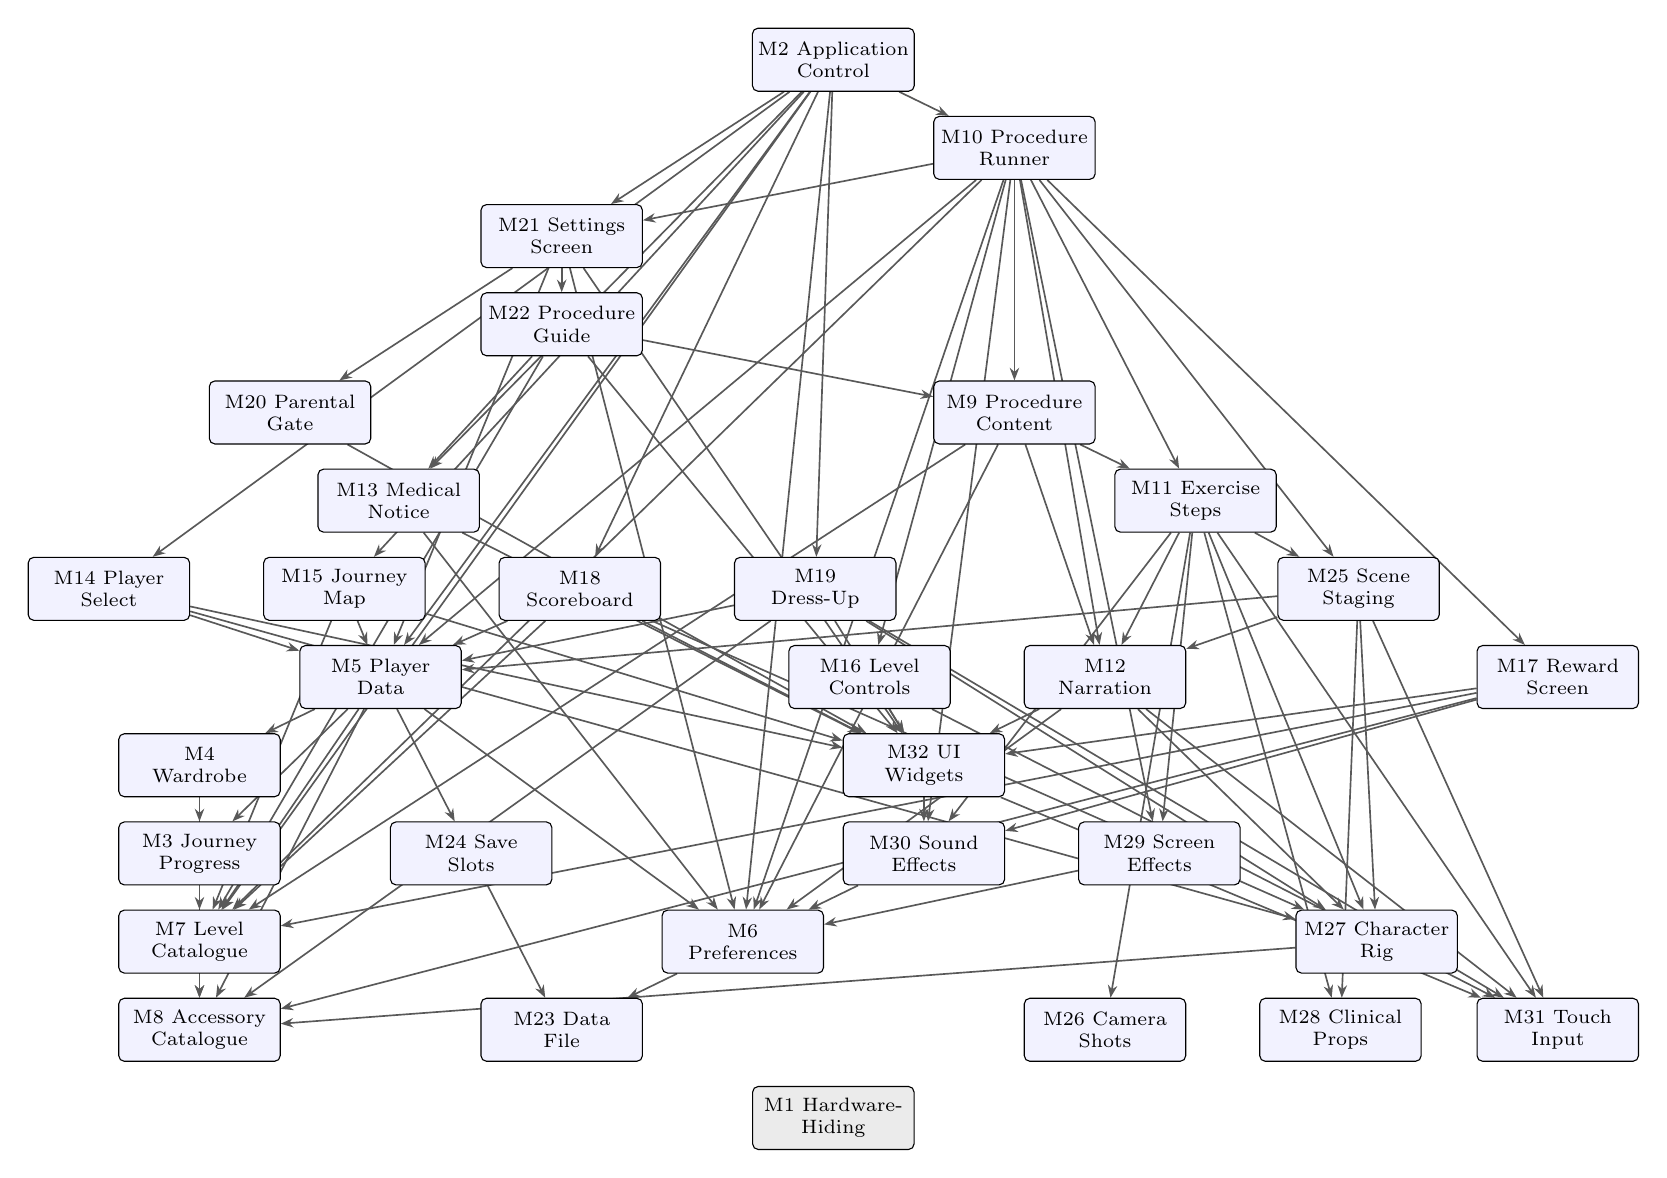
\begin{tikzpicture}[x=2.3cm, y=1.12cm]
% Rows are placed by the longest chain of uses below each module, so every
% arrow points down. Arrows are drawn behind the nodes. Arrows to M1 are left
% out because most modules use it.
\node[mod] (m2)  at (4, 12)   {M2 Application\\Control};
\node[mod] (m10) at (5, 11)   {M10 Procedure\\Runner};
\node[mod] (m21) at (2.5, 10) {M21 Settings\\Screen};
\node[mod] (m22) at (2.5, 9)  {M22 Procedure\\Guide};
\node[mod] (m20) at (1, 8)    {M20 Parental\\Gate};
\node[mod] (m9)  at (5, 8)    {M9 Procedure\\Content};
\node[mod] (m13) at (1.6, 7)  {M13 Medical\\Notice};
\node[mod] (m11) at (6, 7)    {M11 Exercise\\Steps};
\node[mod] (m14) at (0, 6)    {M14 Player\\Select};
\node[mod] (m15) at (1.3, 6)  {M15 Journey\\Map};
\node[mod] (m18) at (2.6, 6)  {M18\\Scoreboard};
\node[mod] (m19) at (3.9, 6)  {M19\\Dress-Up};
\node[mod] (m25) at (6.9, 6)  {M25 Scene\\Staging};
\node[mod] (m5)  at (1.5, 5)  {M5 Player\\Data};
\node[mod] (m16) at (4.2, 5)  {M16 Level\\Controls};
\node[mod] (m12) at (5.5, 5)  {M12\\Narration};
\node[mod] (m17) at (8, 5)    {M17 Reward\\Screen};
\node[mod] (m4)  at (0.5, 4)  {M4\\Wardrobe};
\node[mod] (m32) at (4.5, 4)  {M32 UI\\Widgets};
\node[mod] (m3)  at (0.5, 3)  {M3 Journey\\Progress};
\node[mod] (m24) at (2, 3)    {M24 Save\\Slots};
\node[mod] (m30) at (4.5, 3)  {M30 Sound\\Effects};
\node[mod] (m29) at (5.8, 3)  {M29 Screen\\Effects};
\node[mod] (m7)  at (0.5, 2)  {M7 Level\\Catalogue};
\node[mod] (m6)  at (3.5, 2)  {M6\\Preferences};
\node[mod] (m27) at (7, 2)    {M27 Character\\Rig};
\node[mod] (m8)  at (0.5, 1)  {M8 Accessory\\Catalogue};
\node[mod] (m23) at (2.5, 1)  {M23 Data\\File};
\node[mod] (m26) at (5.5, 1)  {M26 Camera\\Shots};
\node[mod] (m28) at (6.8, 1)  {M28 Clinical\\Props};
\node[mod] (m31) at (8, 1)    {M31 Touch\\Input};
\node[mod, fill=black!8] (m1) at (4, 0) {M1 Hardware-\\Hiding};

\begin{pgfonlayer}{background}
\foreach \a/\b in {
  m2/m5, m2/m6, m2/m7, m2/m10, m2/m13, m2/m14, m2/m15, m2/m18, m2/m19, m2/m21,
  m3/m7, m4/m3, m4/m8,
  m5/m3, m5/m4, m5/m6, m5/m7, m5/m8, m5/m24,
  m6/m23, m7/m8,
  m9/m6, m9/m7, m9/m11, m9/m12,
  m10/m5, m10/m6, m10/m7, m10/m9, m10/m11, m10/m12, m10/m16, m10/m17, m10/m21,
  m10/m25, m10/m29, m10/m30,
  m11/m12, m11/m25, m11/m26, m11/m27, m11/m28, m11/m29, m11/m30, m11/m31,
  m12/m6, m12/m27, m12/m31, m12/m32,
  m13/m6, m13/m32,
  m14/m5, m14/m27, m14/m32,
  m15/m5, m15/m7, m15/m32,
  m16/m31, m16/m32,
  m17/m7, m17/m8, m17/m30, m17/m32,
  m18/m5, m18/m7, m18/m27, m18/m32,
  m19/m5, m19/m8, m19/m27, m19/m31, m19/m32,
  m20/m32,
  m21/m5, m21/m6, m21/m20, m21/m22, m21/m32,
  m22/m7, m22/m9, m22/m13, m22/m32,
  m24/m23,
  m25/m5, m25/m12, m25/m27, m25/m28, m25/m31,
  m27/m8,
  m29/m6, m30/m6,
  m32/m30, m32/m31}
  \draw[use] (\a) -- (\b);
\end{pgfonlayer}
\end{tikzpicture}
\caption[Use hierarchy among modules]{Use hierarchy among modules. An arrow
from A to B means that A uses B. Arrows to \mref{mHH} are not drawn; the modules
that use it are listed in Table~\ref{TblUses}. The figure is vector graphics and
can be zoomed.}
\label{FigUH}
\end{figure}
\end{landscape}

\section{Relationship to the Proof of Concept} \label{SecPoC}

The modules were identified from the Unity project of the 3D proof of concept
(\texttt{src/EyeCanDo} on the \texttt{3d-poc-v2} branch). Table~\ref{TblPoC}
gives, for each module, the PoC classes that implement it today. Paths are
relative to \texttt{Assets/\_Project/Scripts}. Classes under
\texttt{Editor/} build the scenes and content assets, and classes under
\texttt{DevTools/} drive automated smoke tests; neither is part of the released
application, so they are not modules of this design. The studio splash screen
(\texttt{UI/StudioSplash}) is branding with no requirement, and it is kept as
part of the start-up of \mref{mControl}.

\begin{longtable}{p{0.3\textwidth} p{0.6\textwidth}}
\caption{Modules and the Proof-of-Concept Classes That Implement Them}
\label{TblPoC}\\
\toprule
\textbf{Module} & \textbf{PoC classes}\\
\midrule
\endfirsthead
\toprule
\textbf{Module} & \textbf{PoC classes}\\
\midrule
\endhead
\mref{mHH} Hardware-Hiding & Unity engine and OS\\
\mref{mControl} Application Control & \texttt{Core/GameFlow}, the navigation in \texttt{UI/MenuController}\\
\mref{mProgress} Journey Progress & \texttt{Core/Progress/PlayerProgress} (completed levels, coins, \texttt{FinishLevel}), \texttt{Core/Progress/CoinRules}\\
\mref{mWardrobe} Wardrobe & \texttt{PlayerProgress} (\texttt{owned}, \texttt{TryBuy}, \texttt{Equip}), \texttt{Core/Avatar/AvatarLook}\\
\mref{mPlayerData} Player Data & \texttt{Core/GameServices}\\
\mref{mPrefs} Preferences & \texttt{Core/Progress/GameSettings}\\
\mref{mLevels} Level Catalogue & \texttt{Core/LevelCatalog}, \texttt{Core/LevelDefinition}\\
\mref{mAccessories} Accessory Catalogue & \texttt{Core/Avatar/AvatarCatalog}\\
\mref{mContent} Procedure Content & \texttt{Procedure/ProcedureDefinition} and the step assets of each level\\
\mref{mRunner} Procedure Runner & \texttt{Procedure/ProcedureRunner}\\
\mref{mSteps} Exercise Steps & \texttt{Procedure/ProcedureStep}, \texttt{Procedure/Steps/*}\\
\mref{mNarration} Narration & \texttt{UI/NarrationPlayer}, \texttt{UI/CaptionView}, \texttt{Procedure/StoryLine}\\
\mref{mNotice} Medical Notice Screen & not in the PoC\\
\mref{mPlayerSelect} Player Select Screen & \texttt{UI/SaveSelectView}, \texttt{UI/PortraitStudio}\\
\mref{mMap} Journey Map Screen & \texttt{UI/MenuController} (level select), \texttt{UI/LevelCardView}\\
\mref{mHud} Level Controls & \texttt{UI/LevelHud}\\
\mref{mReward} Reward Screen & \texttt{UI/RewardView}\\
\mref{mScoreboard} Scoreboard Screen & not in the PoC\\
\mref{mDressUp} Dress-Up Screen & \texttt{UI/DressUpView}, \texttt{UI/KidSpinner}\\
\mref{mGate} Parental Gate & not in the PoC\\
\mref{mSettings} Settings Screen & \texttt{UI/SettingsView}\\
\mref{mGuide} Procedure Guide Screen & not in the PoC\\
\mref{mDataFile} Data File & \texttt{Core/Progress/DataFile}\\
\mref{mSlots} Save Slots & \texttt{Core/Progress/SaveSlots}\\
\mref{mStaging} Scene Staging & \texttt{Procedure/IProcedureContext}, \texttt{Scene/ExamRoomContext}, \texttt{Scene/SpeakerPortraits}\\
\mref{mCamera} Camera Shots & \texttt{Scene/ShotDirector}\\
\mref{mRig} Character Rig & \texttt{Scene/KidActor}, \texttt{Scene/DoctorActor}, \texttt{Scene/Bean/BeanRig}, \texttt{Scene/Bean/FaceArt}\\
\mref{mProps} Clinical Props & \texttt{Scene/EyeDropRig}, \texttt{Scene/OphthalmoscopeRig}, \texttt{Scene/EyeCloseupRig}, \texttt{Scene/TeachingChart}\\
\mref{mEffects} Screen Effects & \texttt{UI/ScreenEffectsView}\\
\mref{mSound} Sound Effects & \texttt{UI/Sfx}, \texttt{UI/SoundLibrary}\\
\mref{mTouch} Touch Input & \texttt{Scene/Interactable}, \texttt{UI/HoldButton}\\
\mref{mWidgets} UI Widgets & \texttt{UI/ActionButtonsView}, \texttt{UI/ConfirmDialog}, \texttt{UI/OnOffButton}, \texttt{UI/ButtonFeedback}, \texttt{UI/CoinCounter}, \texttt{UI/IdleMotion}, \texttt{Scene/Bobber}, \texttt{Scene/PulseScale}\\
\bottomrule
\end{longtable}

The PoC was built to test the 3D storyboard of one level, and some of its
behaviour differs from the SRS. The design follows the SRS. The following
changes to the PoC are needed, and each one is limited to the modules named:

\begingroup\sloppy
\begin{enumerate}
\item Remove level locking (\texttt{unlockedByDefault},
  \texttt{unlocksOnComplete} and \texttt{unlockedLevels}), so every level can be
  started at any time (\srsfrref{FR_StartLevel}{4}). Affects \mref{mProgress},
  \mref{mLevels} and \mref{mMap}.
\item Record the \emph{in progress} status when a level is started
  (\srsfrref{FR_StartLevel}{4}, \srsfrref{FR_JourneyMap}{3}). Affects
  \mref{mProgress}.
\item Give a level's reward only the first time it is finished. The PoC pays
  \texttt{CoinRules.LevelAgain} coins on every replay, which
  \srsfrref{FR_NoDuplicateReward}{29} forbids. The reward of each level comes
  from its definition (\srsitemref{LC_Rewards}{LC4}) instead of a fixed number of
  coins. Affects \mref{mProgress} and \mref{mLevels}.
\item Apply \emph{finish} in the Procedure Runner when the last step ends,
  instead of inside \texttt{RewardStep}. The celebration moves to
  \mref{mReward}. Affects \mref{mRunner}, \mref{mSteps} and \mref{mReward}.
\item Add restart and hold-to-skip controls to the level controls
  (\srsfrref{FR_RestartLevel}{24}, \srsfrref{FR_NoPenalty}{18},
  \srsfrref{FR_IgnoreRepeatedTouches}{19}). Affects \mref{mHud} and
  \mref{mRunner}.
\item Add a question step that reveals the correct answer
  (\srsfrref{FR_RevealAnswer}{16}), hints after a wrong action
  (\srsfrref{FR_HintOnMiss}{13}), and age-group content
  (\srsfrref{FR_AgeGroup}{7}). Affects \mref{mSteps}, \mref{mContent} and
  \mref{mPrefs}.
\item Add the medical notice, the scoreboard, the parental gate, the procedure
  guide and the nickname (\srsfrref{FR_MedicalNotice}{1},
  \srsfrref{FR_Scoreboard}{30}, \srsfrref{FR_ParentGate}{38},
  \srsfrref{FR_ProcedureGuide}{39}, \srsfrref{FR_Nickname}{40}). These are new
  modules (\mref{mNotice}, \mref{mScoreboard}, \mref{mGate}, \mref{mGuide}) and
  a change to \mref{mPlayerData}.
\item Replace stickers with the reward of the level definition. Affects
  \mref{mProgress} and \mref{mReward}.
\item Add a free character category of accessibility and medical aids
  (glasses, an eye patch, a wheelchair), which the PoC catalogue does not have
  (\srsfrref{FR_DiverseCharacters}{32}). Affects \mref{mAccessories} and
  \mref{mRig}.
\item Keep the development top-up of coins (\texttt{CoinRules.DevCoins}) out of
  release builds, as the PoC already does.
\end{enumerate}
\endgroup

\section{User Interfaces} \label{SecUI}

The user interface is a set of screens opened by the Application Control
Module. Figure~\ref{FigScreens} shows the navigation between them. It matches
the PoC menu scene (title, save files, level select and dress up) and the level
scene, with the screens the SRS adds. The visual design follows the PoC: a 3D
room with the player's character in it, large picture buttons with no words on
the child's screens, and text only in the caregiver area. Every child control
has an icon and a shape as well as a colour (\srsnfrref{NFR_Colour}{10}), and
controls with the same function stay in the same place on every screen
(\srsnfrref{NFR_Layout}{1}).

\begin{figure}[H]
\centering
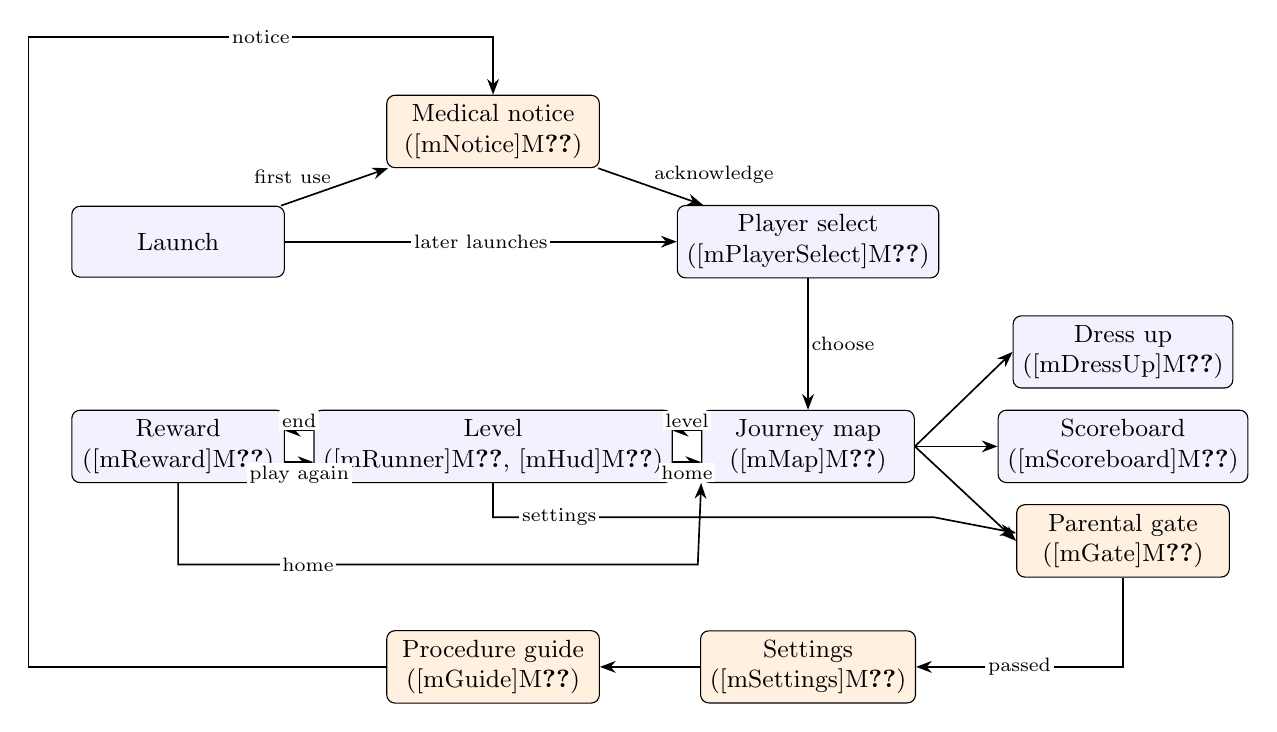
\begin{tikzpicture}[x=1cm, y=1cm,
  scr/.style={draw, rounded corners=3pt, fill=blue!5, font=\small, align=center,
    minimum width=2.7cm, minimum height=0.9cm},
  care/.style={scr, fill=orange!12},
  nav/.style={-{Stealth[length=2mm]}, semithick},
  lbl/.style={font=\scriptsize, align=center, fill=white, inner sep=1pt}]
\node[scr]  (launch)   at (0, 0)      {Launch};
\node[care] (notice)   at (4, 1.4)    {Medical notice\\(\mref{mNotice})};
\node[scr]  (players)  at (8, 0)      {Player select\\(\mref{mPlayerSelect})};
\node[scr]  (map)      at (8, -2.6)   {Journey map\\(\mref{mMap})};
\node[scr]  (level)    at (4, -2.6)   {Level\\(\mref{mRunner}, \mref{mHud})};
\node[scr]  (reward)   at (0, -2.6)   {Reward\\(\mref{mReward})};
\node[scr]  (dress)    at (12, -1.4)  {Dress up\\(\mref{mDressUp})};
\node[scr]  (score)    at (12, -2.6)  {Scoreboard\\(\mref{mScoreboard})};
\node[care] (gate)     at (12, -3.8)  {Parental gate\\(\mref{mGate})};
\node[care] (settings) at (8, -5.4)   {Settings\\(\mref{mSettings})};
\node[care] (guide)    at (4, -5.4)   {Procedure guide\\(\mref{mGuide})};

\draw[nav] (launch) -- node[lbl, above left] {first use} (notice);
\draw[nav] (notice) -- node[lbl, above right] {acknowledge} (players);
\draw[nav] (launch) -- node[lbl] {later launches} (players);
\draw[nav] (players) -- node[lbl, right] {choose} (map);
\draw[nav] ([yshift=2mm]map.west) -- node[lbl, above] {level} ([yshift=2mm]level.east);
\draw[nav] ([yshift=-2mm]level.east) -- node[lbl, below] {home} ([yshift=-2mm]map.west);
\draw[nav] ([yshift=2mm]level.west) -- node[lbl, above] {end} ([yshift=2mm]reward.east);
\draw[nav] ([yshift=-2mm]reward.east) -- node[lbl, below] {play again} ([yshift=-2mm]level.west);
\draw[nav] (reward.south) -- (0, -4.1) -- node[lbl, pos=0.25] {home} (6.6, -4.1) -- (map.south west);
\draw[nav] (map.east) -- (dress.west);
\draw[nav] (map.east) -- (score.west);
\draw[nav] (map.east) -- (gate.west);
\draw[nav] (level.south) -- (4, -3.5) -- node[lbl, pos=0.15] {settings} (9.6, -3.5) -- ([yshift=1mm]gate.west);
\draw[nav] (gate.south) |- node[lbl, pos=0.75] {passed} (settings.east);
\draw[nav] (settings) -- (guide);
\draw[nav] (guide.west) -- (-1.9, -5.4) -- (-1.9, 2.6) -- node[lbl, pos=0.5] {notice} (4, 2.6) -- (notice.north);
\end{tikzpicture}
\caption[Navigation between screens]{Navigation between screens. Caregiver
screens are shaded orange. Every screen returns to the one it was opened from.
After a reset the journey map is shown again; after clearing all data the
medical notice is shown first.}
\label{FigScreens}
\end{figure}

\section{Design of Communication Protocols}

Not applicable. \progname{} communicates with no other system: it has no
server, no network access and no connected hardware (\uref{ucOffline},
\srsnfrref{NFR_Privacy}{28}).

\section{Database Design}

\progname{} has no database. Data is kept in a small number of files in the
storage that the platform keeps private to the application
(\srsnfrref{NFR_DataProtection}{26}): one preferences file for the device, kept
by \mref{mPrefs}, and one player file for each used save slot, kept by
\mref{mPlayerData} through \mref{mSlots}. Each file is written and read by the
Data File Module (\mref{mDataFile}). The files hold only the attributes of the
data dictionary of the SRS (\srsnfrref{NFR_Minimization}{29}):

\begin{itemize}
\item \textbf{Preferences file}: the Local Preferences entity without the
  selected character and the nickname, which belong to a player, together with
  the last player chosen.
\item \textbf{Player file}: the Game Progress and Journey Progress entities
  (the status of each level and the coin balance), the Character Inventory
  entity (owned and worn items, which include the selected character), and the
  nickname.
\end{itemize}

The game content (levels, rewards, steps, narration, accessories) is built into
the application and is never written at run time.

\section{Timeline} \label{SecTimeline}

The modules are built in the phases of the development plan
(\srsdoc{SRS}, Appendix~B). Work on each module is tracked as GitHub issues in
the project repository, where each issue is assigned to one team member.

\begin{center}
\begin{tabularx}{\textwidth}{p{3.6cm} X}
\toprule
\textbf{Phase and dates} & \textbf{Modules}\\
\midrule
Proof of concept\newline 3 Nov.--4 Dec.\ 2026 & Done in the PoC: \mref{mRunner},
\mref{mSteps}, \mref{mNarration}, \mref{mStaging}, \mref{mCamera},
\mref{mRig}, \mref{mProps}, \mref{mEffects}, \mref{mSound}, \mref{mTouch},
\mref{mDataFile}, \mref{mSlots}, and early versions of \mref{mProgress},
\mref{mWardrobe}, \mref{mPlayerData} and \mref{mPrefs}.\\
Core application\newline 5 Dec.\ 2026--18 Jan.\ 2027 & Progress rules of the SRS
in \mref{mProgress} and \mref{mLevels}; \mref{mControl}, \mref{mNotice},
\mref{mMap}, \mref{mHud}, \mref{mReward}, \mref{mPlayerSelect};
\mref{mContent} for the eye-drop level.\\
Feature integration\newline 19 Jan.--11 Feb.\ 2027 & \mref{mScoreboard},
\mref{mDressUp}, \mref{mGate}, \mref{mSettings}, \mref{mGuide},
\mref{mWidgets}; content for the vision-testing and slit-lamp levels.\\
System verification\newline 12 Feb.--8 Mar.\ 2027 & Fixes found by the tests
of the VnV Plan in any module.\\
Final delivery\newline 9 Mar.--6 Apr.\ 2027 & Final art and audio
(\srsitemref{LC_Assets}{LC11}) in \mref{mContent}, \mref{mRig}, \mref{mProps}
and \mref{mSound}.\\
\bottomrule
\end{tabularx}
\end{center}

\section{Generative AI Use Disclosure}

\subsection{AI Tools Used}

\begin{itemize}
\item Claude Opus 5.5 (model \texttt{claude-opus-5-5}), used through Claude Code
  in Visual Studio Code.
\end{itemize}

\subsection{How and Where Used}

\begin{itemize}
\item \textbf{Deriving the decomposition from the PoC.} Claude read the C\#
  sources of the 3D proof of concept, the SRS, the MG and MIS checklists, and
  the course slides on design documents and the MIS, and proposed the
  module decomposition. The team asked for modules that keep the structure
  of the PoC. This affected Sections~\ref{SecMH} and~\ref{SecMD}.
\item \textbf{Drafting text and tables.} Claude drafted the anticipated and
  unlikely changes (Section~\ref{SecChange}), the design decisions
  (Section~\ref{SecConnection}), the traceability matrices
  (Section~\ref{SecTM}), the uses relation and its figure
  (Section~\ref{SecUse}), the comparison with the PoC (Section~\ref{SecPoC}),
  and Sections~\ref{SecUI} to~\ref{SecTimeline}.
\item \textbf{Identifying gaps.} Claude compared the PoC with the SRS and
  listed where the PoC differs from the requirements (Section~\ref{SecPoC}).
\end{itemize}

\subsection{Verification of AI-Generated Content}

\begin{itemize}
\item Every requirement, likely change and unlikely change number was checked
  against the order of the items in the SRS source, and every link uses the
  SRS label of the item it names.
\item Every class named in Table~\ref{TblPoC} and every PoC behaviour named in
  Section~\ref{SecPoC} was checked against the source on the \texttt{3d-poc-v2}
  branch.
\item The uses relation was checked to be acyclic, and Figure~\ref{FigUH} was
  checked against Table~\ref{TblUses}.
\item The document was checked against the course's MG checklist
  (\texttt{docs/Checklists}).
\item \todo{Each team member reviews the modules they will implement and
  confirms the secrets, services and uses before Revision 0.}
\end{itemize}

\newpage{}

\bibliographystyle {plainnat}
\bibliography{../../../refs/References}

\end{document}
